\documentclass[a4paper,12pt]{article}
\usepackage[a4paper,top=1.3cm,bottom=2cm,left=1.5cm,right=1.5cm,marginparwidth=0.75cm]{geometry}

% Пакеты
\usepackage{mathtext} 
\usepackage{setspace}
\usepackage{tabularx}
\usepackage{cmap}
\usepackage{longtable}
\usepackage{icomma}
\usepackage{euscript}
\usepackage{float}
\usepackage{cutwin}
\usepackage{mathrsfs}
\usepackage{adjustbox}
\usepackage{dashbox}
\usepackage[normalem]{ulem}
\usepackage[T2A]{fontenc}			
\usepackage[utf8]{inputenc}                 %!  закрепляет кодировку utf8
\usepackage[english,russian]{babel}         %!  подключает русский и английский
%математические шрифты:
\usepackage{amsmath,amsfonts,amssymb,amsthm,mathrsfs,mathtools} 
\usepackage[colorlinks, linkcolor = purple]{hyperref}      %!  оглавление для панели навигации по PDF-документу + гиперссылки
\usepackage{xcolor}                         %!  добавляет цвета
\usepackage{enumitem}                       %!  задание макета перечня.
\usepackage{xpatch}                         %?  работа с renewcommand и макросами              
\usepackage{cancel}                         %   зачёкивания текста (!!!) для slash-нотации использовать \usepackage{slashed}!!
\usepackage{upgreek}                        %   заглавные греческие буквы
\usepackage{lipsum}                         %?  для вставки кучи текста при форматировании
\usepackage[version=4]{mhchem}              %   химические формулы
\usepackage{multirow}                       %   объединение строк в матрицах
\usepackage{stackengine}                    %   stack символов
\usepackage{tikz}                           %!  рисунки
\usetikzlibrary{positioning}                %?  библиотека для тикза 
\usepackage{titletoc}                       %!  форматирование содержания и заголовков
\usepackage{titlesec}                       %!  форматирование содержания и заголовков
\usepackage{wrapfig}                        %   обтекание таблиц и рисунков
\usepackage{chngcntr}                       %!  для setcounter
\usepackage{fancyhdr}                       %!  для колонтитулов
\usepackage{makecell}                       %?  матрицы с разными выравниваниями и т.п
\usepackage{indentfirst}                    %   добавить indent перед первым 
\usepackage{tocloft}                        %?  изменение названий глав и разделов                       
\usepackage{soul}                           %   типографические примочки, типо зачёркивания и подчёркивания
\usepackage[stable]{footmisc}               %?  продвинутые сноски
\usepackage{subfig}                         %   несколько картинок рядом
   %  задаёт поля страниц

% pgf plots
% \usepackage{pgfplots}
% \pgfplotsset{compat=1.17}

\mathtoolsset{showonlyrefs=true}

%Обозначения теорем и т.п
\theoremstyle{definition}
\newtheorem*{definition}{Определение}
\newtheorem{statement}{Предложение}[section]
\newtheorem{lemma}{Лемма}[section]
\newtheorem{theorem}{Теорема}[section]
\newtheorem*{theoremn}{Теорема}
\newtheorem*{corollary}{Следствие}
\newtheorem*{example}{Пример}
\newtheorem*{note}{Замечание}
\newtheorem*{problem}{Задача}

%Шарабара для содержания и внешнего вида нумерации
\counterwithout{footnote}{section}\DeclareRobustCommand{\divby}{%
	\mathrel{\text{\vbox{\baselineskip.65ex\lineskiplimit0pt\hbox{.}\hbox{.}\hbox{.}}}}%
}



%Толерантный квадратик чтд
%\makeatletter \renewenvironment{proof}[1][\proofname]{\par\pushQED{\qed}\normalfont\topsep6\p@\@plus6\p@\relax\trivlist\item[\hskip\labelsep\bfseries#1\@addpunct{.}]\ignorespaces}{\popQED\endtrivlist\@endpefalse} \makeatother
%\renewcommand\qedsymbol{$\squareulblack$}
%\newcommand{\usubseteq}{\mathbin{\rotatebox[origin=c]{90}{$\subset$}}}
%\DeclareFontEncoding{LS2}{}{\noaccents@}
%\DeclareFontSubstitution{LS2}{stix}{m}{n}
%\DeclareSymbolFont{arrows3}{LS2}{stixtt}{m}{n}
%\DeclareMathSymbol{\squareulblack}{\mathord}{arrows3}{"88}

%Разные операторы и символы
\newcommand{\dotpr}[2]{\bra{#1}\ket{#2}}
\let\AA\relax
%\let\oldvarphi\phi %оно делает так, что \phi становится правильным фи
%\let\phi\varphi
%\let\varphi\oldvarphi
\let\emptyset\varnothing
\DeclareMathOperator*{\esssup}{ess sup}
\DeclareMathOperator*{\ord}{ord}
\DeclareMathOperator*{\supp}{supp}
\DeclareMathOperator*{\pr}{pr}
\DeclareMathOperator*{\Ker}{Ker}
\DeclareMathOperator*{\Vol}{Vol}
\DeclareMathOperator*{\rg}{rk}
\DeclareMathOperator*{\Ima}{Im}
\DeclareMathOperator*{\Alt}{Alt}
\DeclareMathOperator*{\Sym}{Sym}
\newcommand{\eqdef}{\stackrel{\text{\tiny{def}}}{=}}
\newcommand{\pp}{\partial}
\newcommand{\AA}{\mathcal{A}}
\newcommand{\BB}{\mathcal{B}}
\newcommand{\MM}{\mathbb{M}}
\newcommand{\NN}{\mathbb{N}}
\newcommand{\ZZ}{\mathbb{Z}}
\newcommand{\QQ}{\mathbb{Q}}
\newcommand{\RR}{\mathbb{R}}
\newcommand{\CC}{\mathbb{C}}
\newcommand{\FFF}{\mathbb{F}}
\newcommand{\DD}{\mathcal{D}}
\newcommand{\FF}{\mathcal{F}}
\newcommand{\sS}{\mathcal{S}}
\newcommand*\circled[1]{\tikz[baseline=(char.base)]{
		\node[shape=circle,draw,inner sep=2pt] (char) {#1};}}


\title{Исследование взаимной диффузии газов (2.2.1)}
\author{Павлушкин Вячеслав}
\date{\today}


\begin{document}
	
	\maketitle
	
	\section{Аннотация}
	
		\noindent\textbf{Цель работы:} 1) регистрация зависимости концентрации гелия
		в воздухе от времени с помощью датчиков теплопроводности при
		разных начальных давлениях смеси газов; 2) определение коэффициента диффузии по результатам измерений.
		\bigskip
		
		\noindent \textbf{Оборудование:} измерительная установка; форвакуумный насос; баллон с газом (гелий); манометр; источник питания;
		магазин сопротивлений; гальванометр; секундомер.
		
	\section{Теоретические сведения}
	
		Диффузией называют самопроизвольное взаимное проникновение веществ друг в друга, происходящее вследствие хаотичного теплового движения молекул. При перемешивании молекул разного сорта говорят о взаимной (или концентрационной) диффузии.
		
		Диффузия в системе, состоящей из двух компонентов $ a $ и $ b $ (бинарная смесь), подчиняется закону Фика: плотности потока компонентов $ j_{a,b} $ (количество частиц, пересекающих единичную площадку в единицу времени) пропорциональны градиентам их концентраций $ \nabla n_{a,b}$, что в одномерном случае можно записать как
		
		\[ j_a = -D\dfrac{\partial n_a}{\partial x}, \quad j_b = -D\dfrac{\partial n_b}{\partial x}, \]
		где $ D $ -- коэффициент взаимной диффузии компонентов. Знак <<минус>> отражает тот факт, что диффузия идёт в направлении выравнивания концентраций. Равновесие достигается при равномерном распределении вещества по объёму сосуда ($ \partial n / \partial x = 0 $).
		
		В случае работы с данной установкой можно считать, что диффузионный поток одинаков в любом сечении трубки, соединяющей сосуды $V_1$ и $V_2$. Следовательно:
		
		\begin{align}
			J = -DS\dfrac{n_1-n_2}{l} \qquad DS\frac{n_1-n_2}{l} = -V_1\dfrac{dn_1}{dt} = V_2\dfrac{dn_2}{dt} \\
			\dfrac{dn_1 - dn_2}{dt} = -\dfrac{n_1-n_2}{l}DS\left(\dfrac{1}{V_1}+\dfrac{1}{V_2}\right) \quad\Rightarrow\quad n_1-n_2 = (n_1-n_2)_0e^{-\dfrac{t}{\tau}}
		\end{align}
		
		В данной работе исследуется взаимная диффузия гелия и воздуха. Давление P и температура T в условиях опыта предполагаются неизменными: $ p=(n_{He}+n_{\text{в}})kT $, где $ n_{He} $ и $ n_{\text{в}} $ -- концентрации (объёмные плотности) диффундирующих газов. Поэтому для любых изменений концентраций справедливо $ \Delta n_{He}=-\Delta n_{\text{в}} $. Следовательно, достаточно ограничиться описанием диффузии одного из компонентов, например гелия $ n_{He} $:
		
		\begin{equation}\label{1}
				j_{He}=-D\dfrac{\partial 	n_{He}}{\partial x}.
		\end{equation}
		
		Приведём теоретическую оценку для коэффициента диффузии. В работе концентрация гелия, как правило, мала $ (n_{He} \ll n_\text{в}) $. Кроме того, атомы гелия существенно легче молекул, составляющих воздух ($ \mu_{He} \ll \mu_{O_2}, \mu_{N_2} $), значит и их средняя тепловая скорость велика по сравнению с остальными частицами. Поэтому перемешивание газов в работе можно приближенно описывать как диффузию примеси лёгких частиц $ He $ на практически стационарном фоне воздуха. Коэффициент диффузии в таком приближении равен
		
		\begin{equation}\label{2}
			D=\dfrac{1}{3}\lambda 	\overline{v},
		\end{equation}
		
		где $ \overline{v}=\sqrt{\frac{8RT}{\pi \mu}} $ -- средняя тепловая скорость частиц примеси, $ \lambda = \frac{1}{n_0\sigma} $ -- их длина свободного пробега, $ n_0 $ -- концентрация рассеивающих центров (фона), $ \sigma $ -- сечение столкновения частиц примеси с частицами фона.
		
		Таким образом, теория предсказывает, что коэффициент диффузии бинарной смеси обратно пропорционален давлению в системе $ D \propto 1/P $, и не зависит от пропорций компонентов, что и предлагается проверить в работе экспериментально.
		
	\section{Экспериментальная установка}
	
		Для исследования взаимной диффузии используется следующая установка:
		
		\begin{wrapfigure}{l}{8cm}
			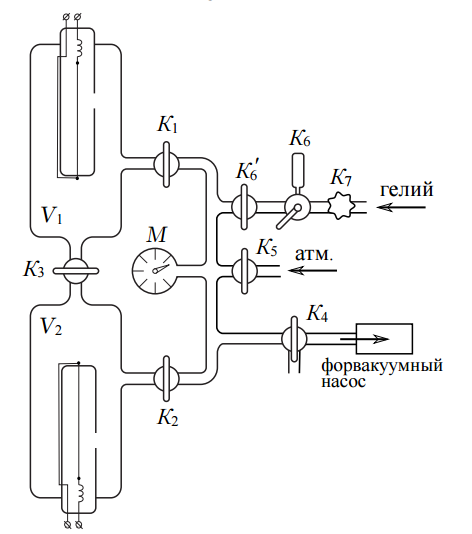
\includegraphics[scale=0.8]{facility}				
			\caption{Схема установки}
			\label{facility}
		\end{wrapfigure}
		Здесь $V_1,\; V_2$ -- два сосуда с примерно равным объемом, в которые мы будем загонять воздух и гелий.
		
		Данная конструкция позволяет провести диффузию, которая возможна только при равенстве давлений.
		
		Основное оборудование, с помощью которого мы будем снимать измерения -- датчики теплопроводности, через которые пропускают ток. Они подключены к мосту, который позволяет нам устанавливать начальное равновесное состояние.
		
		При изменении концентрации в колбах вольтметр покажет нам разность напряжений на датчиках, что, из-за их конструкции, означает разность концентраций. 
		
		С помощью изменения напряжения мы и будем изучать процесс диффузии, т.к. во время ее протекания концентрации газов начинают устанавливаться, что заметно на графике разницы напряжений от времени.
		
	\section{Ход работы}
	
		\subsection{Коэффицент взаимной диффузии}
		
		Для смеси гелий-воздух исследуем зависимость коэффициента взаимной диффузии о начального давления в системе. Для этого будем фиксировать с помощью компьютера в лаборатории зависимость показаний вольтметра от времени, прошедшего с начала эксперимента. Проверим то, что процесс диффузии подчиняется закону: \[U = (U)_0e^{-\dfrac{t}{\tau}}.\]
		
		Для этого построим графики зависимости в виде:
		\begin{align}
			 \ln(U) = \ln(U_0) + (-\tau^{-1})t \Rightarrow \ln\left(\frac{U_0}{U}\right) = \frac{t}{\tau}
		\end{align}
		
		\begin{figure}[h!]
			\centering
			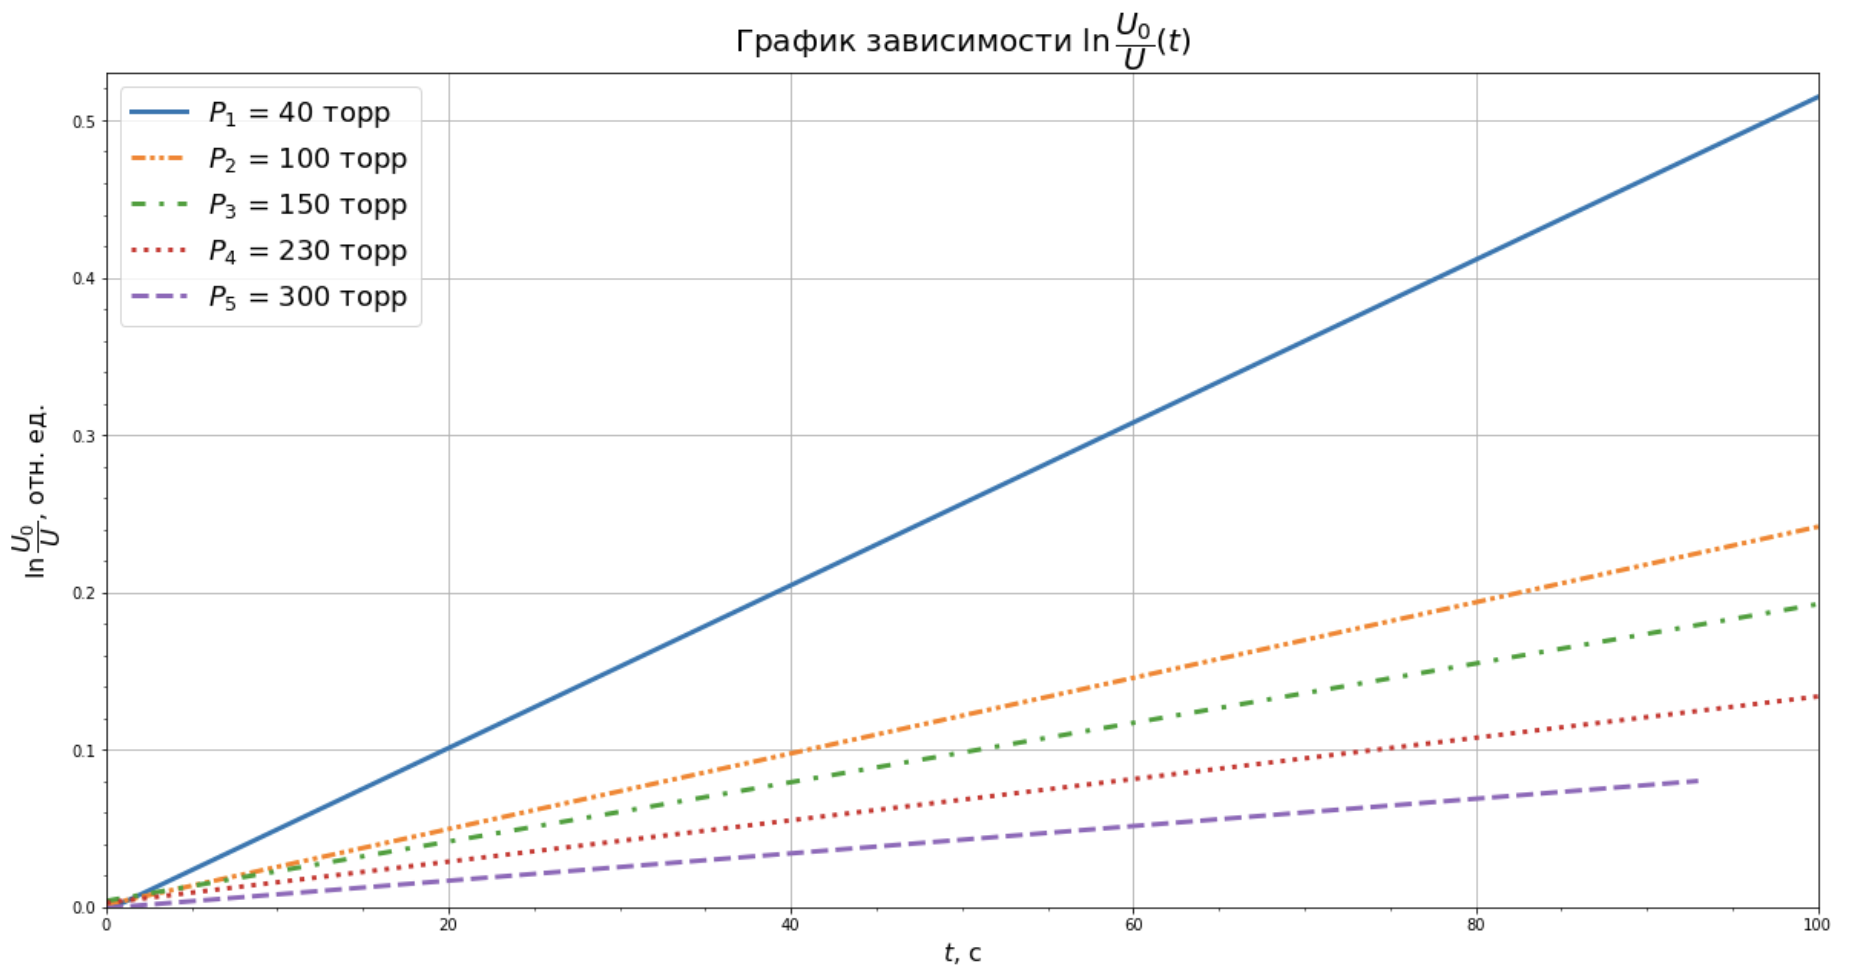
\includegraphics[scale=0.542]{graph1}
			\caption{Зависимость $ \ln\frac{U_0}{U} $ от $ t $}
			\label{graph}
		\end{figure}
	
		График \eqref{graph} линеен, следовательно у нас происходит действительно диффузия. Далее мы можем найти $\tau$ как коэффицент наклона. Находить будем по МНК. В нашем случае $\ln\frac{U_0}{U} = k t$, и $k = \frac{1}{\tau}$.
		
		\begin{equation}
			k=\frac{\langle t\cdot \ln \frac{U_0}{U} \rangle - \langle t\rangle \langle \ln \frac{U_0}{U}\rangle}{\langle t^2 \rangle - \langle t \rangle^2} 
		\end{equation}
		\begin{equation}
			\sigma_k^\text{случ}=\frac{1}{\sqrt{N}}\sqrt{\frac{\langle \left(\ln\frac{U_0}{U}\right)^2 \rangle - \langle \ln\frac{U_0}{U} \rangle^2}{\langle t^2 \rangle - \langle t \rangle^2} - k^2  }
		\end{equation}
		\begin{equation}
			\sigma_k^{\text{сист}} = k\varepsilon_k =  k\cdot\sqrt{\varepsilon_{U_0}^2 + \varepsilon_U^2 + \varepsilon_t^2} = k\cdot\sqrt{\left(\frac{\sigma_{U_0}}{U_0}\right)^2+ \left(\frac{\sigma_{U}}{U}\right)^2 + \left(\frac{\sigma_t}{t}\right)^2} 
		\end{equation}
		\begin{equation}
			\sigma_k = \sqrt{\left( \sigma_k^\text{случ} \right)^2 + \left( \sigma_k^\text{сист} \right)^2 }
		\end{equation}
	
		Очевидно, что $\varepsilon_\tau = \varepsilon_k$.
		
		Проведем рассчеты для каждого значения давления, получим таблицу:
		\bgroup
		\def\arraystretch{1.3}%
		\begin{table}[H]
			\centering
			\begin{tabular}{|c|c|c|c|c|c|}
				\hline
				$ P $, торр & $ \sigma_P $, торр & $ k \cdot 10^{-3} $, с$ ^{-1} $ & $ \sigma_{k} \cdot 10^{-3} $, с$ ^{-1} $ & $ \tau $, с & $ \sigma_\tau $, с \\ \hline
				40 & 1,9 & 5,172 & 0,075 & 193,35 & 2,80 \\ \hline
				100 & 1,9 & 2,402 & 0,034 & 416,32  &5,89  \\ \hline
				150& 1,9 & 1,886 & 0,027 & 530,22 &7,59  \\ \hline
				230 & 1,9 & 1,312 & 0,019 & 762,20  & 11,04 \\ \hline
				300 & 1,9 & 0,868 & 0,012 & 1152,07 & 15,93 \\ \hline
			\end{tabular}
			\caption{Аппроксимация зависимостей}
			\label{tab:approx}
		\end{table}
		\egroup
		
		Далее посчитаем коэффициенты взаимной диффузии для различных давлений по формуле:
		\begin{align}
			D = \frac{1}{\tau}\frac{VL}{2S} & & \sigma_D = D\sqrt{\varepsilon_\tau^2 + \varepsilon_V^2  + \varepsilon_{\frac{L}{S}}^2}
		\end{align}
		Параметры моей установки: $V = (775\pm 10)\text{ см}^3$, $\dfrac{L}{S} = (5,3\pm 0,1)\text{ }\dfrac{1}{\text{см}}$. 
		
		Посчитаем $D\text{ и }\sigma_D$:
		
		\bgroup
		\def\arraystretch{2}%
		\begin{table}[H]
			\centering
			\begin{tabular}{|c||c|c|c|c|c|}
				
				\hline
				$ P $, торр & 40&100&150&230&300\\
				\hline
				$ D $, $\dfrac{\text{см}^2}{\text{с}}$ & 10,62& 4,93& 3,87&2,69&1,78 \\
				\hline
				$ \sigma_D $, $\dfrac{\text{см}^2}{\text{с}}$ & 0,29& 0,13 & 0,10& 0,07&0,05\\
				\hline
			\end{tabular}
			\caption{Значения коэффициента диффузии при различных давлениях}
			\label{tab:D}
		\end{table}
		\egroup
		
		\subsection{График зависимости $D(\dfrac{1}{P})$}
		
		\begin{figure}[H]
			\centering
			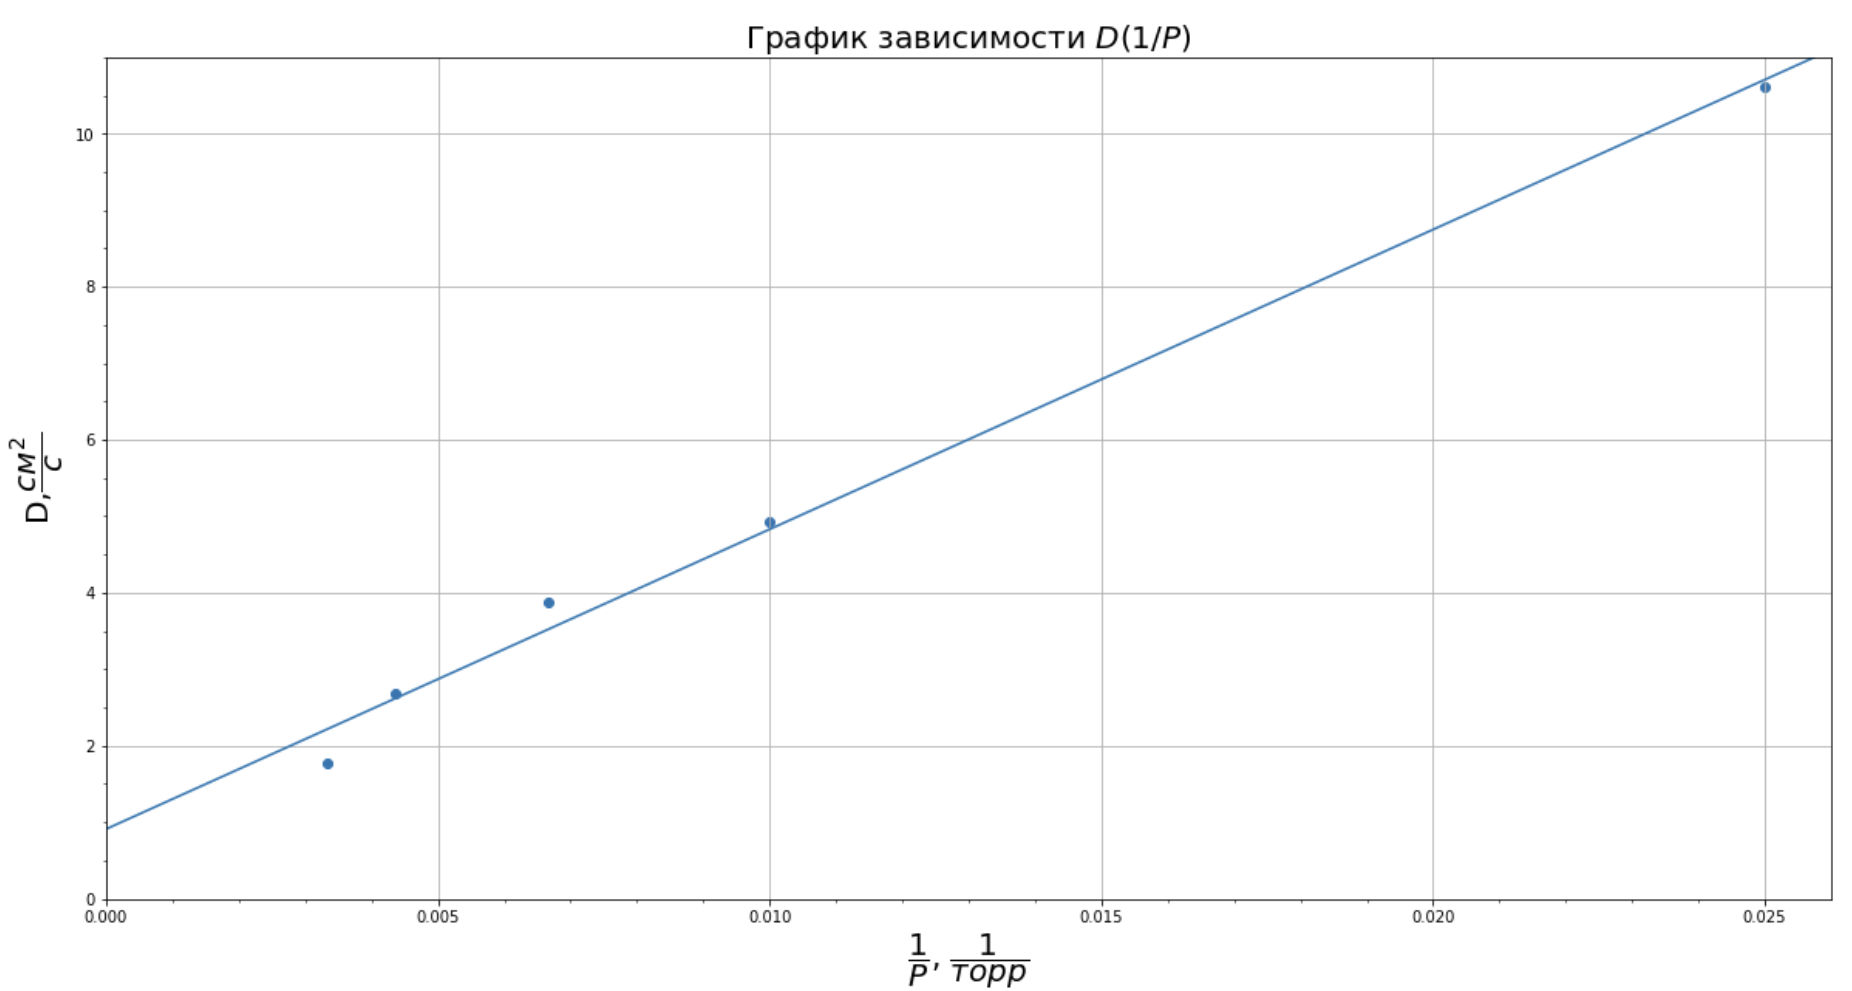
\includegraphics[scale=0.543]{graph2}
			\caption{Зависимость $ D $ от $ \dfrac{1}{P} $}
			\label{graph2}
		\end{figure}
	
		Построен по МНК, коэффицент наклона $k = (391,9\pm18,9)\text{ } \frac{\text{см}^2}{\text{с}\cdot\text{торр}}$. 
		
		Значит, коэффициент диффузии при атмосферном давлении можно найти таким образом:\[D_\text{атм} = k\dfrac{1}{P_\text{атм}} = (0,516\pm0,03)\text{ } \frac{\text{см}^2}{\text{с}}\]
		
		\subsection{Длина свободного пробега}
		
		По полученным данным оценим длину свободного пробега атомов гелия в воздухе:
		
		\begin{align}
			D=\dfrac{1}{3}\lambda\langle v\rangle,\text{ где } \langle v \rangle = \sqrt{\dfrac{8RT}{\pi \mu}} \Rightarrow \lambda = 3D\sqrt{\dfrac{\pi \mu}{8RT}} \approx 131,4\text{ нм}
		\end{align}
		
	\section{Вывод}
	
		В ходе работы:
		
		\begin{itemize}
			\item Была зарегистрирована зависимость концентрации гелия в воздухе от времени с помощью датчиков теплопроводности при различных начальных давлениях смеси газов.
			\item По результатам измерений был определен коэффицент взаимной диффузии для смеси гелий-воздух: $D_\text{атм} = (0,516\pm0,03)\text{ } \frac{\text{см}^2}{\text{с}}$, что совпадает по порядку величины с табличными данными: $D_\text{табл} = 0,62\text{ } \frac{\text{см}^2}{\text{с}}$.
			\item Была оценена длина свободного пробега гелия в воздухе: $\lambda = (131,4\pm7,6)\text{ нм}$, что опять-таки сходится с табличными данными по  порядку величины: $\lambda_\text{табл} = 175\text{ нм}$. 
		\end{itemize}
		Основная доля ошибок приходится на барометр, и тот факт, что мы не можем полностью точно сбалансировать мост (он очень легко расстраивается).
		
		
	
	
\end{document}

